%\documentclass[times]{MGS_class}
%
%\title{Self Publishing}
%\author{Lukas Frühstück, BSc \textsuperscript{1} and Jakob Schade, BSc \textsuperscript{1}}
%
%\begin{document}
%
%\twocolumn[{\csname @twocolumnfalse\endcsname
%	\begin{center}
%	\maketitle
%	
%	\noindent \scriptsize \textsuperscript{1}\textsl{UAS Technikum Vienna, Game Engineering and Simulation, Vienna, AUT}\\
%	
%	\end{center}
%	
%	\hspace{15mm}
%}]

\begin{abstract}
As an independent game developer a successful launch of a game it especially crucial. The task of self-publishing may sound easy but there can be significant challenges. Different platforms and manufacturers have different rules and requirements which have to be met when releasing a game for their system. The following paper explores which options are available for an indie-developer to release their game, how big the challenges for different gaming platforms are and what general strategies should be kept in mind.
\end{abstract}


\begin{keywords}
self-publishing, indie-developer, PC, Steam, iOS, Android, consoles
\end{keywords}


\section{Introduction} 
\label{sec:introduction}
The classical way of releasing a newly developed game involves a publisher who has the resources and necessary industry contacts to quickly distribute a game over many platforms using different distribution channels. However, as an independent developer without any publisher it can be significantly harder to successfully release a game on many different platforms. On the other hand, without a contract with a publisher the developer retains complete control over his game and is free to decide about its fate.

Over the last years more and more indie-game studios started self-publishing their games. On the PC it is comparatively simple to achieve this. On consoles on the other hand it can be more difficult as the manufacturer enforces certain requirements and has to agree that your game can be published. The rules imposed on developers vary between different target platforms. Some are very restrictive whereas others allow the developer more freedom.

With the ongoing trend of indie-games most console manufactures have created special programs for developers to allow self-publication. This significantly simplified the release process but it is still more difficult compared to self-publication on the PC. 

Self-publishing on mobile platforms is, compared to gaming consoles, also comparatively simple. One of the big difficulties here is that especially for the main platforms, Apple and Android, the market is very oversaturated and it can be hard to get the game recognized and discovered by players


\section{PC}
\label{sec:pc}
The PC is a very versatile platform with many different ways to distribute a finished game. Nowadays the primary way for indie-developers to release a game on PC is to use the various available online distribution platforms that are available. Distribution with physical media is still common for games but it is generally not feasibly for small developers due the required financial expenses.

\subsection{Steam}
\label{subsec:steam}
When someone thinks about purchasing and downloading a game for pc, steam is probably the number one store where most of the gamers would start to search for their favored game. On steam you can find nearly any game, but what is the reason that so many publisher or game developer decide to release their games on Valve Corporation's platform?

When steam started in 2003 it was a platform to play Valve's own games on Windows PCs. Since then it grows and grows. Over the years more and more publisher decided to release their games with steam which currently has a userbase of more than 125 million users.

\begin{figure}[!hbp]
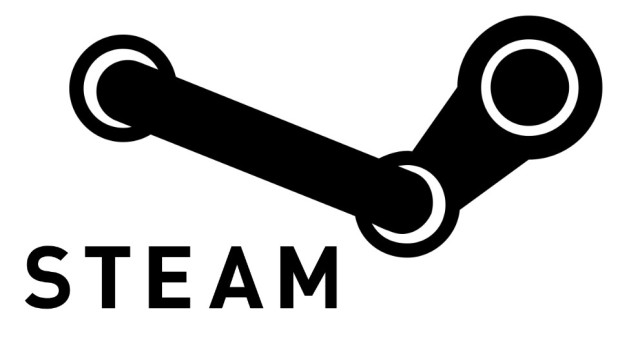
\includegraphics[width=\linewidth]{img/steam.jpg}
\centering
\caption{ Steam Logo }
\label{fig:steam}
\end{figure}

While this sounds nice it may be a problem to get the attention for the game. Steam currently offers more than 4500 games as the announced on GDC 2015. The get some attention for a game or to get it in steam store primarily it has to go through the Greenlight process, where gamer can decide if they would buy a game if it would be released in the store. But more on this later. \citep{smith_valve_2015}

\subsubsection{Publishing Guidelines}
\label{steam_publishing_guidelines}
To publish a game on Steam you have to own the rights to sell the game or have a specific authorization to represent the developers. Porn, inappropriate or offensive content, warez or leaked content is not allowed. The game must not allow cheating or hacking. Also games using copyright materials such as assets without permission from the owner are not allowed.
In Greenlight process soliciting, begging, auctioning, selling, advertising, referrals racism, discrimination as well as threats of violence or harassment, even as a joke, are strictly forbidden. \citep{valve_steam_2016}


\subsubsection{Costs}
\label{subsec:steam_costs}
To get access to submit a game to steams Greenlight you have to pay a one-time Greenlight submission fee. The amount of the fee is 90 euro and is fully donated to Child's Play, a charity dedicated to improving the lives of children in over 70 hospitals worldwide. Once paid, this steam account is allowed to post and update an infinite amount of games or software within the Greenlight process. \citep{valve_steam_2016}

Steam does not officially talk about additional costs. In the official announcement they write that they will get in contact with the developer to talk about revenue. Some unofficial reports say that steam receives about 40\% of the prize of the final game.

\subsubsection{Pricing Model}
\label{subsec:steam_pricing}
Steam offers many different pricing models. In the official Steamworks documentation valve writes that they will get in contact with the developer to find the best price for the game.

If a game is in store the publisher has the possibility to set a discount for the game. Mostly they are only for a limited time available. It is also possible to combine games and release them as packs with a little discount. Also an old game as additional content is part of the possibilities. To promote the game the developer has also the right to offer it for free.

\subsubsection{Steamworks}
\label{subsec:steam_steamworks}
Steamworks is a platform inside Steam. You can provide additional possibilities for your customers when they connect your game with their steam account. \citep{valve_steamworks_2016}

Steamworks supports matchmaking, achievements, anti-cheat technology, micro-transaction and is available for free for download and for retail games.

Steamworks also says that it is very easy to be implemented into a nearly ready game and brings not much overhead with.
More information about Steamworks can be found here: https://www.steampowered.com/steamworks/

\subsubsection{Greenlight}
\label{subsec:steam_greenlight}
Greenlight was started in summer of 2012. It is a possibility for small and new developers to present their games for a small fee. Than Steam community members have the chance to support game ideas they like and make it possible for the developers to release it in store.


\subsection{GOG}
\label{subsec:gog}
GOG.com, formerly Good old Games, is a distribution service for DRM free games and movies. It was originally founded in 2008 to sell classic games which are not further available in retail stores. In 2012 they changed their market and started to sell more recent title too.

\begin{figure}[!hbp]

\includegraphics[width=\linewidth]{img/gogcom.png}
\centering
\caption{ GOG.com Logo }
\label{fig:gog}
\end{figure}

Comparing GOG.com with different online distributer is a little bit difficult, because main stream titles are not their main selling point. But on some specific games they are the second best behind Steam if they are not event better than Valve's platform.

Until today GOG.com has more than 1300 games in its library and they become more every week.

\subsubsection{Publishing Guidelines}
\label{gog_publishing_guidlines}
Every game will be reviewed by itself. The GOG.com Team will get in contact with every developer who submits a game and will tell them, what they think about their game.

\subsubsection{Costs}
\label{subsec:gog_costs}
There are no one-time costs at GOG.com when a new game is submitted to their indie platform. The revenue of all sold Games is split between GOG.com and the developer. GOG.com receives 30\% of the earnings.

\subsubsection{Get in Contact}
\label{subsec:gog_contact}
To get a game into the GOG.com store the developers have to submit it on the indie website of GOG.com (http://www.gog.com/indie). GOG.com will get in touch with the developers to discuss if the game has a change to be released. They say from themselves that they will respond to every request and if they reject a game, they will tell the developers exactly why they decided so.

Important for GOG.com is, that the game is DRM free. Else there is no chance that the game will be released on their website. Also all contents of the game have to be originally made by the developers themselves or at least the developers have to hold all rights for assets etc.

Each and every game will be rated for itself if it is worthwhile to get a place in GOG.com store. The distributer says “We're not machines. We talk.” Every game will get its individual evaluation. \citep{gog_gog.com_2016}


\subsection{Humble}
\label{subsec:humble}
The Humble Store is well known because of the Humble Bundle. But aside from this cheap bundles they also provide download games or codes for steam. Humble Bundle was launched in 2010 but it took three additional years until the Humble Store itself went online. According to the Humble Bundle team, they "wanted to create something that would allow developers to easily sell their games through their own web site as well as provide a painless buying experience for purchasers". \citep{kuchera_penny_2013}

\begin{figure}[!hbp]

\includegraphics[width=\linewidth]{img/humble.png}
\centering
\caption{ Humble Store Logo }
\label{fig:humble}
\end{figure}

\subsubsection{Store or Widget?}
\label{subsec:humble_store_or_widget}
There are two different ways for selling a game via Humble Bundle. The developers can choose to offer the game in the humble store, where many different games are available. But they can also decide to sell the game from an own website. Therefore Humble Bundle provides a widget which can be used to be implemented in the games online appearance. \citep{humble_bundle_humble_2016}

\subsubsection{Store}
\label{humble_store}
The Humble Store is the "normal" distribution medium. The game will be available alongside other games. The games can be provided either as steam keys or as DRM free downloads. To submit a game the developers have to fill out to form on this site (https://www.humblebundle.com/developer/ store/application). The Humble Bundle Team will get in touch with the developers to discuss details.

\paragraph{Costs}\mbox{}\\
The developers receive 75\% of the revenue, which does not mean that Humble Bundle gets 25\%. They just keep 15\% and the other 10\% go to charity. There are no one-time costs at Humble Bundle. \citep{humble_bundle_humble_2016}

\subsubsection{Widget}
\label{humble_widget}
The Humble Widget on the other side is more or less a possibility for the developers to sell their games themselves. After a registration on the Humble Bundle website the developers get some code to sell the game directly from its website. \citep{humble_bundle_humble_2016-1}

\paragraph{Costs}\mbox{}\\
The Costs for this options are very low. Humble Bundle only wants 5\% of the revenue if the developers sell the game outside of the Humble Store.

Humble Bundle says about itself that the want to support the developers. They don't want much revenue and offer many different methods to distribute the game. Downside is, that not every distribution model is 

\subsubsection{Pricing Model}
\label{humble_pricing_model}
Humble Bundle offers Humble Pricing. The developers can choose if they want to use it. It automatically calculates different currency values and rounds them up to get more beautiful prices.

In the backend they also have full control over possible discounts for their games.

The Humble Bundle Team says itself that they want to support the developers. Humble store as well as Humble Widget offer really good revenues for the developer. To use all possibilities like sell Steam keys the game has to be submitted on the other distribution platform to, which could be a little bit more difficult than releasing on Humble Bundle.


\subsection{Windows Store}
\label{subsec:windows_Store}
Windows Store is Microsoft's answer to Apple's App Store or Google's Play Store. But while the second and the third primarily offer mobile apps, the Windows Store shall also distribute PC Games especially from indie developers. Windows Store was first published with the Consumer Preview of Windows 8 in February 2012. Since then every new Microsoft operating system received a version of it. In 2015, together with the launch of Windows 10, the Xbox and the Windows Phone stores were merged together into the Windows Store. \citep{microsoft_publish_2016}

\begin{figure}[!hbp]
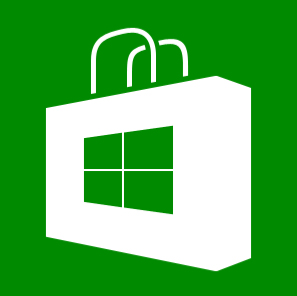
\includegraphics[width=\linewidth]{img/windows-store.png}
\centering
\caption{ Windows Store Logo }
\label{fig:windows}
\end{figure}

There are currently more than 669.000 apps available in the Store and because every new Windows Version is delivered with a preinstalled version of it, there is a gigantic userbase.

\subsubsection{Costs}
\label{windows_costs}
To sign up, new developers have to pay a one-time fee to grand access. For indie developers the amount is 19\$. A company account has to pay 99\$. These allow to publish apps on Windows NT and Windows Mobile Store.

Students are supported through the Dreamspark program.
Microsoft also splits the revenue of the sold apps. They keep 30\% of the income and pay the other 70\% to the developers.

\subsubsection{Pricing Models}
\label{windows_pricing_model}
The developers can choose if they want to offer their app for free or for a specific price. If they decide for the second one, there are many other options to choose from.

For example it is possible to offer a free trial of the game or application. Also the developers are allowed to choose a market where they want to sell their game and decide on own prices for them.

Offering a discount is also a possibility.

\subsubsection{Analytics}
\label{windows_analytics}
Aside from the frontend of the Windows Store, Microsoft offers a developer portal, where the developers can watch over their published apps. There they can find a summary and a detailed report about downloads, sales, finances, ratings, etc.

It is also possible to lay filter over this information. For example it is possible to get specific information for a single region.

Format
Windows Store supports Win32 Application or .NET-Framework Applications. These can be packed for distribution in Windows store. For this is Microsoft Application Virtualization (short App-V) used to allow sandboxing.

Windows Store is a little bit different than the other three presented stores. It is more similar to the mobile platforms, that will be shown further in this paper.

\section{Mobile}
\label{sec:mobile}
Publishing apps and games on the common mobile platforms Android and Apple iOS is comparatively easy. Both platforms provide app stores which allow developers to submit their apps. 
The biggest challenge when releasing a mobile game is not publishing it. The difficult part is to stand out and gain public exposure in a market with millions of other apps and games.

\subsection{Apple App Store}
\label{subsec:apple_app_store}
The Apple App Store is the apps and games marketplace for Apple's mobile devices, primarily the iPhone and iPad. The store hosts over 1,2 million apps \citep{ranger_ios_2015} and counts more than 100 billion app downloads. \citep{ingraham_apples_2015} 

Apple's App Store is one of the key factors that caused the boom of mobile applications and mobile games. Founded in 2008 it gained enormous popularity with the success of the iPhone. 

Nowadays the market is oversaturated with many different games and it can be very hard to get attention. Even if the odds of achieving financial success on the App Store are very small, it can be well worth it, should a game be included in one of the store's featured lists. At this point it is easily possible to get many downloads and to gain huge earnings. 

\begin{figure}[!hbp]
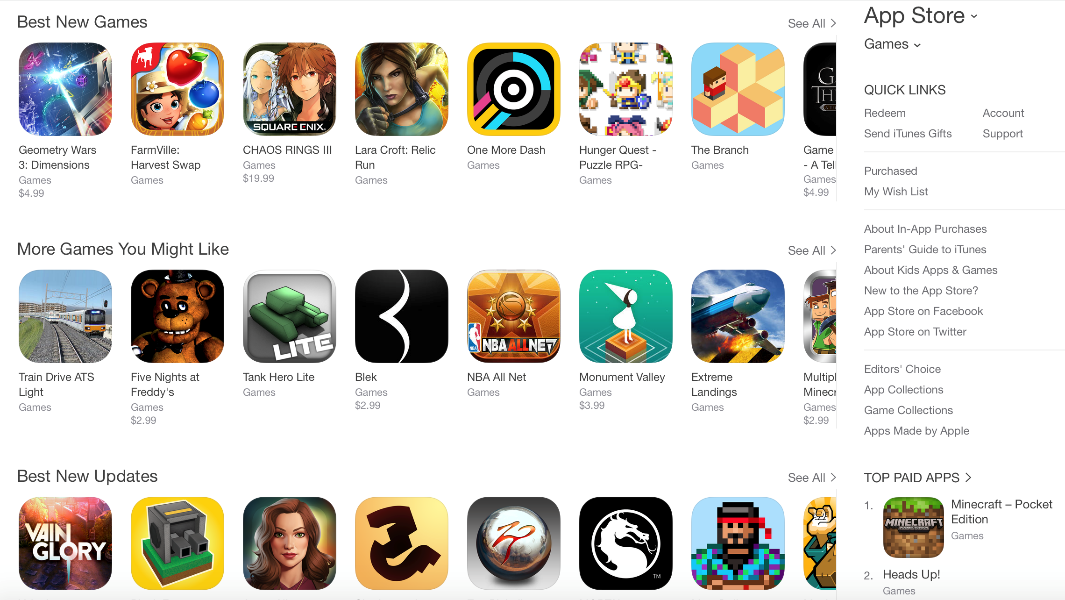
\includegraphics[width=\linewidth]{img/apple.png}
\centering
\caption{ Apple App Store overview}
\label{fig:apple}
\end{figure}

\subsubsection{Publishing Guidelines}
\label{subsec:ios_guidelines}
To publish a game on iOS an Apple Developer Account is necessary. With this account it is possible to submit any app to the App Store. However, before it will be released the game is reviewed by Apple and if it does not meet their criteria it will not be published. The process of reviewing a new App can take multiple days and has to be considered when planning a release. 

Apple is very strict about their rules and does not allow certain types of content on their store. The exact content guidelines are rather loosely defined in "We will reject Apps for any content or behavior that we believe is over the line." \citep{apple_app_2016}, but in general it can be said that games containing pornography, racism, certain types of violence, certain religious themes or personal attacks are likely to being rejected.

Additionally, if the game looks like "it was cobbled together in a few days" \citep{apple_app_2016} or does not do "something useful, unique or provides some form of lasting entertainment" \citep{apple_app_2016} it will be rejected too.

\subsubsection{Costs}
\label{subsec:ios_costs}
Developing apps and games for iOS is free but publishing them on the App Store requires joining the Apple Developer Program which incurs an annual fee of \$99 for either a private person or an organization.\citep{apple_choosing_2016}

Additionally, Apple keeps 30\% of the revenue a game or an app generates – either through direct sales of In-App purchases. \citep{apple_apple_2016}

\subsubsection{Pricing Models}
\label{subsec:ios_pricing_models}
The Apple App Store allows for different business and pricing models to monetize a game. The most straightforward one is to publish a game as a premium app which requires the customer to pay for it once when downloading it. After that he can play the game without restrictions on his devices.

It is also possible to release a free app. This can be used for example to create a demo version which gives the customer the option to try the game an encourage him to buy the full premium version.

Another option is In-App purchases which can be used to sell premium upgrades, special items, consumables and many other digital goods directly in the app. This pricing model can be hugely successful. For example, in 2015 the game developer Bethesda generated profits of more than \$5 million with their free game "Fallout Shelter" which contained one single item as an In-App purchase. \citep{tassi_fallout_2015}

The final pricing option is to publish a free app which contains advertisements and generates revenue this way. There are many different types of ads that can be integrated into an app – from simple banners to big full screen popups and even video clips. These ads are provided by different advertising programs. Notable examples for this are Apple's own iAd and Google AdMob. The revenue generated by in-app advertisements can vary drastically and depends on the advertising provider, on the number of users an app has and on the number of users that click on the advertisements.  

\subsubsection{Promotions}
\label{subsec:ios_promotions}
Apple will choose and promote games that they like by putting them on the front page of the App Store, by integrating them in lists of featured apps in certain categories of by giving out awards like the "Apple Design Award". The process of getting an app promoted cannot be influenced by the developer but it can be crucial for the success of a game on the platform.

As an example: The game "Blek", developed by the Austrian brothers Denis and Davor Mikan, was released in December 2013. It received general favorable reviews and sold about 30.000 copies in the first 2 months. Then it received the "Apple Design Award 2014" and got featured on the store's front page. In the following two months additional 500.000 copies were sold. \citep{borison_blek_2014}

\paragraph{Promo Codes}\mbox{}\\
Apple provides also the capability to generate promo codes for an app or for in-app items which can be used in custom marketing campaigns to promote a game.

\subsubsection{Apple Game Center}
\label{subsec:ios_game_center}
As an additional feature for games published on the App Store, Apple provides the “Game Center”. It is a social gaming platform with features like multiplayer, friend invites, leaderboards and achievements. The Game Center can be used by any game on the App Store free of charge. \citep{apple_game_2016}

\subsubsection{Apple GameKit}
\label{subsec:ios_game_kit}
The GameKit framework works in conjunction with the Game Center. It provides peer-to-peer network multiplayer functionality for phones connected via Bluetooth or WiFi in the same local area. Furthermore, it also contains functionality for an in-game voice chat system which can be implemented in games. \citep{apple_gamekit_2016}

\subsection{Android}
\label{subsec:android}
When publishing games for devices running Android different things have to be considered in comparison to Apple iOS. Android is a open ecosystem with more than 24.000 \citep{opensignal_android_2015} different device models. The primary publishing platform for most of these device is the official Android Play Store from Google. But as Android is an open platform, other distribution channels are allowed too and there are devices out there that have only access to third part distribution platforms and not the official store. To reach as many Android users as possible, these options have to be considered.

\subsubsection{Play Store}
\label{subsec:android_play_store}
The Play Store was founded in 2008 and is the official distribution channel for apps, games and other digital goods on the Android platform. It is developed and hosted by Google and contains about 1,4 million apps \citep{ranger_ios_2015} with more than 200 billion total downloads. \citep{protalinski_app_2016}

As with the Apple App Store these numbers show that the market is heavily oversaturated and it is difficult to gain enough attention to become popular and financially successful. 

\begin{figure}[!hbp]
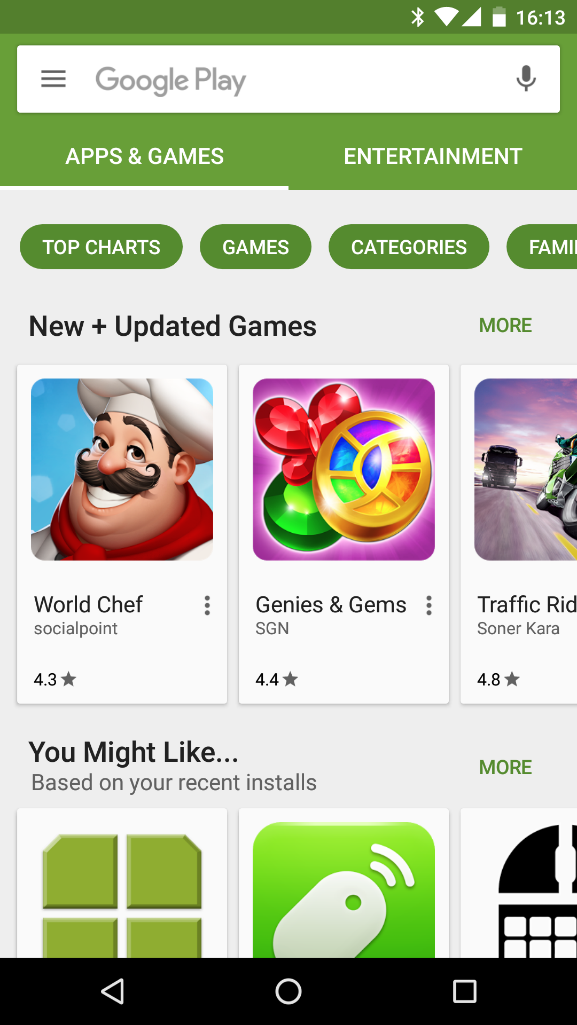
\includegraphics[height=\linewidth]{img/android.png}
\centering
\caption{ Android Play Store overview}
\label{fig:android}
\end{figure}

\paragraph{Publishing Guidelines}\mbox{}\\
To publish a game on the Play Store a Google Developer Account is necessary. With this account it is possible to submit any app to the Play Store. 

The general criteria for apps and games that are allowed on the Play Store are similar to those on the Apple App Store. No explicit sexual content, violence, bullying and hate speech are allowed.

However, the process of submitting a new app is generally much faster compared to the Apple App Store as the Play Store does not have a lengthy review process. But this does not mean that apps are not reviewed before being published on the Play Store. Before 2015 all new apps were immediately accepted but since then a half-automated process is in place that checks new apps before making them available on the store. \citep{perez_app_2015}

\paragraph{Costs}\mbox{}\\
To create an Android Developer Account an initial, one-time fee of \$25 is required. Additionally, 30\% of the revenue generated by app sales and in-app products go to Google.

\paragraph{Pricing Models}\mbox{}\\
Similar to the Apple App Store, the Play Store supports four different pricing models. 

Premium apps are sold for a price determined by the developer. Once bought they are available on all devices of the customer.

Free apps can be released too. These could be used as demo app or combined with an ad provider like Google AdMob to create revenue by displaying advertisements. In-App payments for items, consumables or other game related products are supported too.

\paragraph{Promotions}\mbox{}\\
The Play Store provides auto generated charts and lists of apps which are currently trending. Additionally, Google provides high quality apps and games with an “Editor’s Choice” award which causes an app to be included in a separate section of the Play Store.

As with the App Store, it can be crucial for the success of a game to be included in one of the lists of features games. This highly increases the visibility of the game in the otherwise extremely oversaturated Play Store. 

Generating promo codes is also supported and allows for custom promotional campaigns.

\subsubsection{Google Play Games Services}
\label{subsec:android_play_services}
The Google Play Games Services is a framework of tools and libraries that can be added to a mobile game. While created by Google and thus mainly focused on Android and the Play store, it is also available for iOS, C++ and Unity.

The framework is provided free of charge and consists of many different features which can be integrated into a game and are focused primarily around social gaming. \citep{hartrell_unlocking_2014}

\paragraph{Social Features}\mbox{}\\
Social features included in the library are for example leaderboards, achievements, player stats, events, game invites and sending gifts to friends. 

\paragraph{Multiplayer}\mbox{}\\
The Play Games Services include libraries that enable multiplayer capabilities for games. Real time and turn based multiplayer games modes are supported without the requirement for a special server or connection management. \citep{google_play_2016}

\paragraph{Other}\mbox{}\\
Additional features include a piracy protection and license check to ensure the user is playing a legitimate copy of the game and the ability to store save games online to allow the user to easily move between devices without losing progress.

One of the newest features added in October 2015 is the ability for users to quickly create Let's Play videos of their mobile games and share them on social media. \citep{perez_android_2015}

\subsubsection{Amazon App Store}
\label{subsec:amazon_app_store}
The Amazon App Store is an alternative distribution platform for android apps and games. With over 400.000 apps it is the second largest store for Android behind the official Play Store. \citep{rubin_amazon_2015} It comes preinstalled on Amazon's own Android devices like the Kindle Fire tablet, where it is the only available app store, and can be installed on most other Android devices. As a special future Amazon offers promotional campaigns like "Free App of the Day" which provides users with a different free app every day.
 
The registration for the Amazon App Store is free and the basic revenue share is similar to other stores where 30\% of the income goes to Amazon. New apps on the Amazon App Store have to undergo a manual review process similar to the one on Apple's App Store.

\paragraph{Concerns}\mbox{}\\
While the Amazon App Store has gained significant market share, it might not be the right distribution platform for a mobile game. The terms of services of Amazon contain certain wordings which caused the International Game Developers Association to call it "…a threat to game developers". \citep{igda_amazons_2011}

Clauses in the developer agreement include the ability for Amazon to temporarily reduce the price of an app up to 80\% of the minimum list price during promotions without asking or notifying the developer. Additionally, developers have to agree to not make an exclusive promotional deal with any other app store. \citep{igda_amazons_2011}

These terms and conditions might change over time and it is important for a developer to carefully check them before releasing their game on this store.

\subsubsection{SlideMe}
\label{subsec:slideme}
SlideMe is another alternative app distribution platform for Android. The SlideMe store is preinstalled on devices of over 140 manufacturers and is focused on niche markets where Google Play is not available. \citep{about_2016} 

The registration as a developer on SlideMe is free and their business model is also based on the common 70/30\% revenue share system.  

SlideMe focuses on high quality apps without an oversaturation of the market and without useless apps. Due to this, SlideMe uses a strict review process for new apps. 

Being listed on the SlideMe store can help to boost the sales of a new app and especially small developers report better sale than on Google Play. \citep{hill_indie_2015}

\subsubsection{Android Game Consoles}
\label{subsec:android_game_consoles}
Android as an open platform is also used in other devices than phones and tablets. There are some Android based game consoles out there with their own stores. While they are not as widespread as smartphones and tablets, their customer base consists primarily of gamers and thus publishing for these systems might be worthwhile. 

\paragraph{Razer Forge TV}\mbox{}\\
\begin{figure}[!hbp]
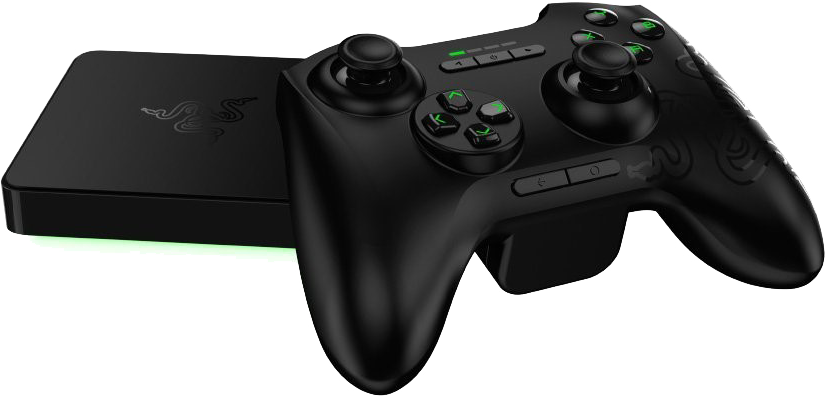
\includegraphics[width=\linewidth]{img/razer.png}
\centering
\caption{ Razer Forge TV }
\label{fig:razer}
\end{figure}
In 2012 the Android-based gaming console called “Ouya” was funded on Kickstarter. \citep{ouya_2016} While it was one of the first of its kind, it did not achieve long term success and was discontinued and sold to Razer in 2015. Razer rebranded it and build a new hardware platform called the “Razer Forge TV” and added a new App Store called the “Cortex Store”. \citep{razer_2016}

Creating a developer account for this platform is free and all sales use the typical revenue share where Razer receives 30\%.

\paragraph{NVidia SHIELD}\mbox{}\\
\begin{figure}[!hbp]
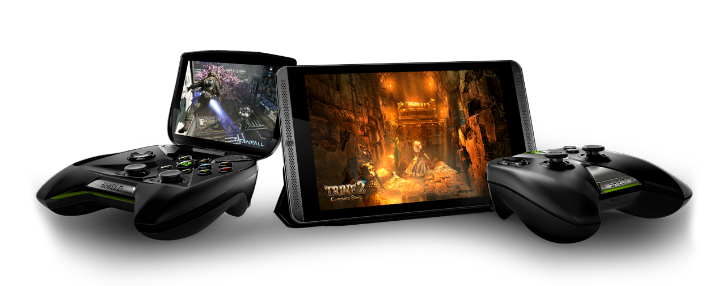
\includegraphics[width=\linewidth]{img/shield.png}
\centering
\caption{ NVidia SHIELD lineup }
\label{fig:shield}
\end{figure}
NVidia SHIELD is a line of Android devices focused on gaming. They are developed and manufactured by NVidia and possess a higher that average gaming performance. 

Currently there are three SHIELD devices available: A handheld console, a tablet with wireless controller and a TV console and streaming box. \citep{next_generation_2016}

Games for the NVidia SHIELD devices are sold through the Google Play Store and thus the same rules and regulations apply. However, the SHIELD devices also contain a separate app which features and highlights specific games and links to their Play Store pages. The list of games in this application is curated by NVidia and focuses on high quality games, especially those which use the hardware capabilities available on SHIELD devices.  To be included in this list an application has to be sent to NVidia where the game will be reviewed. 

The process of releasing for SHIELD does not incur any other costs than the registration fee and the revenue share of the Google Play Store.

\section{Consoles}
\label{sec:consoles}
Developing for a gaming console is much more difficult than for PC. But the reason is not that the developer has to learn a new programming language or work with difficult systems, it is because of the guidelines provided by the console manufactures which have to be followed

These guidelines are several hundred pages long and contain many information how a game for this specific console has to look like, how the game should react on specific user input and how not. The game developer is not allowed to reinvent the wheel, he must follow the guidelines strictly else the game would not be released on the console. This process can take several months up to half of a year and many games fail to be released on a console. Mostly the developers were not able to implement them into their games or were not able to finance the additional time which was needed to do this.

One easy to understand example for this guidelines is the button layout. On a Nintendo console the A-Button is used to accept an action and the B-Button to decline it. On Microsoft's console, the Xbox, it is similar. The difference is that the buttons are on different positions. Nintendo A-Button is on the right side while Microsoft's is on the bottom side of the layout. That would not be a problem if there was not Sony. Son's guidelines do not just say this button is for action and this is for decline, it differs depending on the region where the game will be released. So the developer has to implement a switch in the code to change the button layout if it is released in Japan or in Europe or America. In detail this means that in Europa and America the gamers accept actions with the X-Button on the PlayStation controller. This works with the same layout like Microsoft's Xbox controller. In Japan actions are accepted with the Circle-Button on the right side of the controller. So it is similar to the Nintendo controller where the "accept"-Button is also on the right side.

These guidelines go quite into detail and the developers have to follow all and everything of them to be able to release a game on a console. But the console manufactures have started to think about independent developers and to support them a little bit.

In the following part it can be read about what it takes to release a game on a specific console and where information and help can be found to reach this goal.

\subsection{Nintendo}
\label{subsec:nintendo}
Nintendo is a very traditional Japanese corporation. They have strictly hierarchical order and work very conservative. But in the last few years they began to open up for more and more developer and after the launch of their online shops they also started to support independent developer to release their games on Nintendo's consoles.

With the Nintendo Wii U they created a possibility for easy entry into development for their console. Every licensed Nintendo developer is allowed to use either the Nintendo Web Framework or Unity for Wii U to develop and publish their games but more on this later.

\begin{figure}[!hbp]
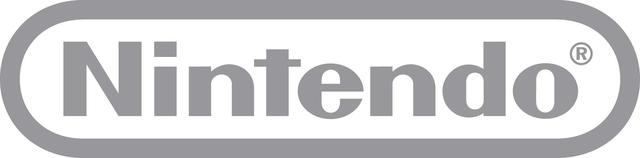
\includegraphics[width=\linewidth]{img/nintendo.jpg}
\centering
\caption{ Nintendo Logo }
\label{fig:nintendo}
\end{figure}

If a developer wants to develop a game for Nintendo's consoles he has to register on www.warioworld.com. This is the main developer platform of Nintendo. If he wants to use the aforementioned Nintendo Web Framework or Unity for Wii U, he also has to sign up on wiiu-developers.nintendo.com to get access to the needed software.

Before developers are allowed to release a game on Nintendos online shops they must be rated with an age rating certificate. They will need the ESRB for North American releases and PEGI as well as USK for the European ones. The game itself must not contain many different languages but the electronic manual, which is attended to all releases, must contain English, French, Italian, German, Spanish and Dutch.

The trickiest part is the QA check, which we have already addressed before. Nintendo tests quite fast, but after they find a few bugs in the game or the documentation, they send it back to the developers and they have to start the deploying process all over again. And they are not allowed to forget to update the version number of all their papers documentaries.

30\% of the income goes directly to Nintendo. But since the eShop launched on Wii U and 3DS the developer or publisher have the free choice to choose how much the game will cost. Also they are allowed to create temporary price drops and develop a good price strategy. \citep{hill_indie_2015}

\subsection{Playstation}
\label{subsec:playstation}
Sony was the first one of the "big" three companies which started to support independent developer with their program called PSP Mini. That program was built especially for small developer to help them with their first releases and lower the financial risks with offering a monthly revenue. Today still the company supports startups and university to produce games for PlayStation.

\begin{figure}[!hbp]

\includegraphics[width=\linewidth]{img/ps4.png}
\centering
\caption{ Sony Playstation 4 Logo }
\label{fig:ps4}
\end{figure}

For European developer there is one specific website, where they have to register to get in touch with the Sony Team which is responsible for Europe, Australia and a few small countries. On http://develop.scee.net/ everything can be found, what it takes to be a Sony PlayStation developer. \citep{hill_indie_2015}

If the game will be approved for Sony's online store depends on their scope and the implemented platform features. Sony exclusive game titles must include at least one platform feature. All non-exclusive title must maintain feature and content parity for at least three months.

\subsection{Xbox}
\label{subsec:xbox}

\begin{figure}[!hbp]

\includegraphics[width=\linewidth]{img/xbox.png}
\centering
\caption{ Microsoft XBox One Logo }
\label{fig:xboxone}
\end{figure}
At the beginning of Xbox One, Microsoft decided to lock indie developers out from their console. But only a short time after launch, they made a U-turn and support them now too. \citep{hill_indie_2015}

Microsoft started ID@Xbox to allow qualified game developer to release their games in Xbox store. ID also allows developer to use the Xbox Live features. These connect all gamers together over all Microsoft platforms. Xbox Live is also supported by Windows Store applications. So games which are released on Xbox and Windows Store can be connected and are able to exchange data.

With ID@Xbox it is possible for the developers to get all the benefits out of the console, including the full power of the console, cloud services, Kinect and Xbox Live toolset such as Xbox SmartGlass, multiplayer, Achievements, Gamerscore and more.

Register to the program is easy, just fill out a form on http://www.xbox.com/en-us/Developers/id. Everyone can register, but developers who can show some previous work on PC or other consoles have a far higher chance to be accepted. But once in there is much benefit the developers can gain from Microsoft.

%
%\bibliographystyle{apalike-url}
%\bibliography{Bibliography-SelfPublishing}

%\end{document}
